\documentclass{beamer}
\pdfstringdefDisableCommands{%
  \def\\{}%
  \def\texttt#1{<#1>}%
}
\beamertemplatenavigationsymbolsempty


% Footnote
\setbeamertemplate{footline}{\leavevmode%
  \begin{beamercolorbox}[wd=.33\paperwidth,left,ht=2.5ex,dp=1.5ex,rightskip=4pt plus 1pt, leftskip=4pt]{subsection in head/foot}
    Team 12
  \end{beamercolorbox}%
  \begin{beamercolorbox}[wd=.33\paperwidth,center,ht=2.5ex,dp=1.5ex]{section in head/foot}
  \end{beamercolorbox}%
  \begin{beamercolorbox}[wd=.34\paperwidth,ht=2.5ex,dp=1.5ex,leftskip=4pt plus 1pt,rightskip=4pt plus 1pt]{subsection in head/foot}
    \hfill\insertframenumber/\inserttotalframenumber
  \end{beamercolorbox}%
}


\title{Stato di avanzamento}
\subtitle{Sprint 2}
\author{
  \texorpdfstring{\parbox{45mm}{\centering\scriptsize Zaid Cheikh Ibrahim \\[-0.3em] {\tiny PO Operativo}}}{} \and 
  \texorpdfstring{\parbox{45mm}{\centering\scriptsize Tian Cheng Xia \\[-0.3em] {\tiny Scrum master}}}{}\\[1em]
  \texorpdfstring{\parbox{45mm}{\centering\scriptsize Qun Hao Henry Lee \\[-0.3em] {\tiny Developer}}}{} \and 
  \texorpdfstring{\parbox{45mm}{\centering\scriptsize Manuel Paris \\[-0.3em] {\tiny Developer}}}{}\\
}
\institute{
  Corso di Ingegneria del Software\\
  Alma Mater Studiorum $\cdot$ Università di Bologna  
}
\date{14 novembre 2022}


\begin{document}

{
\setbeamertemplate{footline}{} 
\begin{frame}
  \titlepage
\end{frame}
}
\addtocounter{framenumber}{-1}

\begin{frame}
  \frametitle{Obiettivi dello sprint}
  \begin{itemize}
    \item Permettere di selezionare il numero di tweet da raccogliere con una singola richiesta
    \item Implementare la ricerca dei tweet per intervallo temporale
    \item Realizzare la ricerca dei tweet per parola chiave
    \item Visualizzare su mappa i dati di geolocalizzazione dei tweet
    \item Implementare la raccolta di tweet in tempo reale
  \end{itemize}
\end{frame}

\begin{frame}
  \frametitle{Use case}
  \begin{figure}
    \centering
    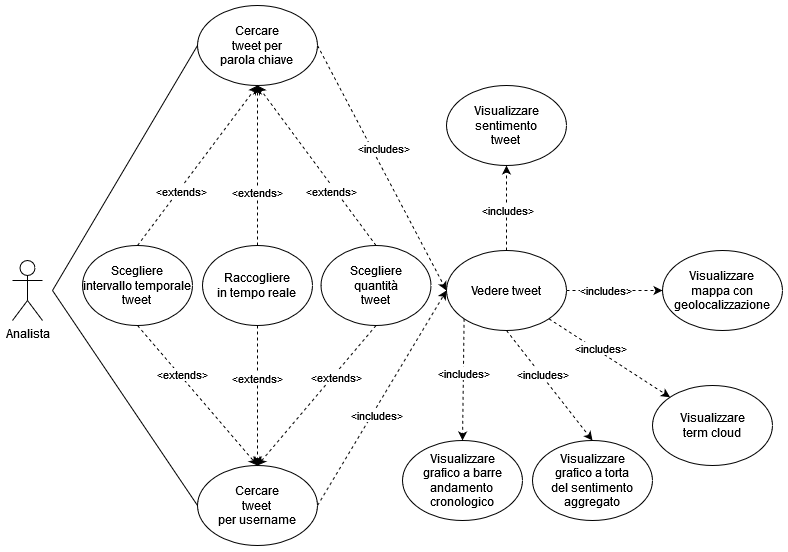
\includegraphics[width=\textwidth]{./img/usecase.png}
  \end{figure}
\end{frame}

\begin{frame}
  \frametitle{Pre-retrospettiva}
  \begin{figure}
    \centering
    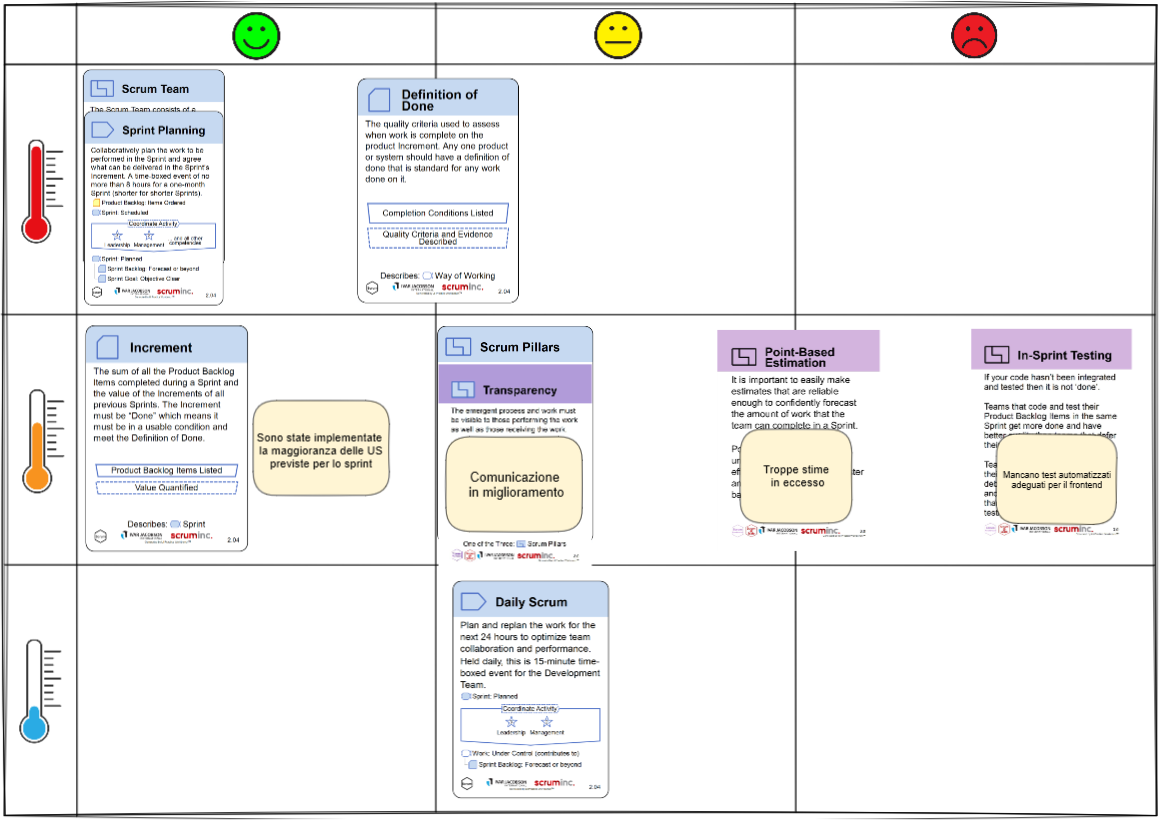
\includegraphics[width=\textwidth]{./img/preretrospettiva.png}
  \end{figure}
\end{frame}

\begin{frame}
  \frametitle{Stato attuale}
  \begin{itemize}
    \item Ricerca dei tweet per parola chiave
    \item Possibilità di scegliere il numero di tweet da raccogliere con una richiesta
    \item Filtrare per intervallo temporale dei tweet
  \end{itemize}
  \begin{figure}
    \centering
    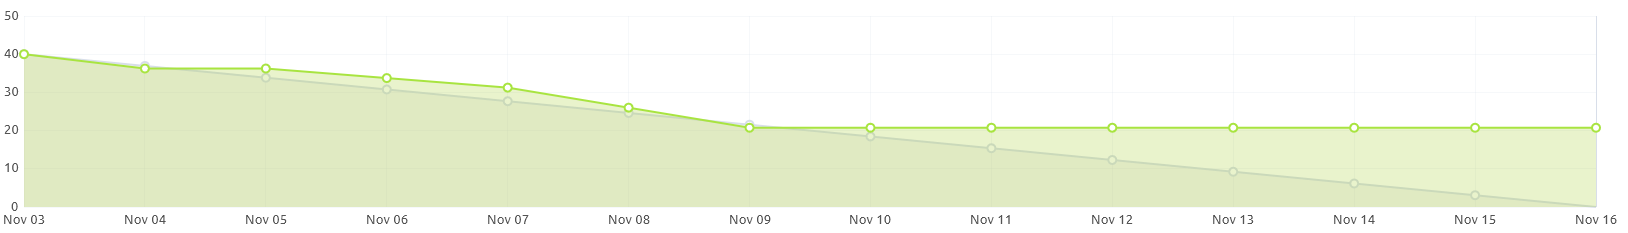
\includegraphics[width=\textwidth]{./img/burndown.png}
    \caption{Burndown sprint 2}
  \end{figure}
\end{frame}

\end{document}